%description: Basic Document in English
%% Based on a TeXnicCenter-Template by Tino Weinkauf.
%%%%%%%%%%%%%%%%%%%%%%%%%%%%%%%%%%%%%%%%%%%%%%%%%%%%%%%%%%%%%

%%%%%%%%%%%%%%%%%%%%%%%%%%%%%%%%%%%%%%%%%%%%%%%%%%%%%%%%%%%%%
%% HEADER
%%%%%%%%%%%%%%%%%%%%%%%%%%%%%%%%%%%%%%%%%%%%%%%%%%%%%%%%%%%%%
\documentclass[a4paper,twoside,10pt]{report}
% Alternative Options:
%	Paper Size: a4paper / a5paper / b5paper / letterpaper / legalpaper / executivepaper
% Duplex: oneside / twoside
% Base Font Size: 10pt / 11pt / 12pt


%% Language %%%%%%%%%%%%%%%%%%%%%%%%%%%%%%%%%%%%%%%%%%%%%%%%%
\usepackage[USenglish]{babel} %francais, polish, spanish, ...
\usepackage[T1]{fontenc}
\usepackage[ansinew]{inputenc}
%\usepackage{hyperref}
\usepackage{lmodern} %Type1-font for non-english texts and characters
\usepackage{float}

%% Packages for Graphics & Figures %%%%%%%%%%%%%%%%%%%%%%%%%%
\usepackage{graphicx} %%For loading graphic files
%\usepackage{subfig} %%Subfigures inside a figure
%\usepackage{pst-all} %%PSTricks - not useable with pdfLaTeX

%% Please note:
%% Images can be included using \includegraphics{Dateiname}
%% resp. using the dialog in the Insert menu.
%% 
%% The mode "LaTeX => PDF" allows the following formats:
%%   .jpg  .png  .pdf  .mps
%% 
%% The modes "LaTeX => DVI", "LaTeX => PS" und "LaTeX => PS => PDF"
%% allow the following formats:
%%   .eps  .ps  .bmp  .pict  .pntg


%% Math Packages %%%%%%%%%%%%%%%%%%%%%%%%%%%%%%%%%%%%%%%%%%%%
\usepackage{amsmath}
\usepackage{amsthm}
\usepackage{amsfonts}
\usepackage{multirow}
\usepackage{caption}

%% Line Spacing %%%%%%%%%%%%%%%%%%%%%%%%%%%%%%%%%%%%%%%%%%%%%
%\usepackage{setspace}
%\singlespacing        %% 1-spacing (default)
%\onehalfspacing       %% 1,5-spacing
%\doublespacing        %% 2-spacing


%% Other Packages %%%%%%%%%%%%%%%%%%%%%%%%%%%%%%%%%%%%%%%%%%%
\usepackage{a4wide} %%Smaller margins = more text per page.
%\usepackage{fancyhdr} %%Fancy headings
%\usepackage{longtable} %%For tables, that exceed one page
\usepackage{hyperref}
\usepackage[hyperpageref]{backref} 

%%%%%%%%%%%%%%%%%%%%%%%%%%%%%%%%%%%%%%%%%%%%%%%%%%%%%%%%%%%%%
%% Remarks
%%%%%%%%%%%%%%%%%%%%%%%%%%%%%%%%%%%%%%%%%%%%%%%%%%%%%%%%%%%%%
%
% TODO:
% 1. Edit the used packages and their options (see above).
% 2. If you want, add a BibTeX-File to the project
%    (e.g., 'literature.bib').
% 3. Happy TeXing!
%
%%%%%%%%%%%%%%%%%%%%%%%%%%%%%%%%%%%%%%%%%%%%%%%%%%%%%%%%%%%%%

%%%%%%%%%%%%%%%%%%%%%%%%%%%%%%%%%%%%%%%%%%%%%%%%%%%%%%%%%%%%%
%% Options / Modifications
%%%%%%%%%%%%%%%%%%%%%%%%%%%%%%%%%%%%%%%%%%%%%%%%%%%%%%%%%%%%%

%\input{options} %You need a file 'options.tex' for this
%% ==> TeXnicCenter supplies some possible option files
%% ==> with its templates (File | New from Template...).



%%%%%%%%%%%%%%%%%%%%%%%%%%%%%%%%%%%%%%%%%%%%%%%%%%%%%%%%%%%%%
%% DOCUMENT
%%%%%%%%%%%%%%%%%%%%%%%%%%%%%%%%%%%%%%%%%%%%%%%%%%%%%%%%%%%%%
\begin{document}

\pagestyle{empty} %No headings for the first pages.


%% Title Page %%%%%%%%%%%%%%%%%%%%%%%%%%%%%%%%%%%%%%%%%%%%%%%
%% ==> Write your text here or include other files.

%% The simple version:
\title{CIRA as a Cloud Service}
\author{Vivek Agrawal}
%\date{} %%If commented, the current date is used.
\maketitle

%% The nice version:
%\input{titlepage} %%You need a file 'titlepage.tex' for this.
%% ==> TeXnicCenter supplies a possible titlepage file
%% ==> with its templates (File | New from Template...).


%% Inhaltsverzeichnis %%%%%%%%%%%%%%%%%%%%%%%%%%%%%%%%%%%%%%%
\tableofcontents %Table of contents
\cleardoublepage %The first chapter should start on an odd page.

\pagestyle{plain} %Now display headings: headings / fancy / ...



%% Chapters %%%%%%%%%%%%%%%%%%%%%%%%%%%%%%%%%%%%%%%%%%%%%%%%%
%% ==> Write your text here or include other files.

%\input{intro} %You need a file 'intro.tex' for this.


%%%%%%%%%%%%%%%%%%%%%%%%%%%%%%%%%%%%%%%%%%%%%%%%%%%%%%%%%%%%%
%% ==> Some hints are following:

\chapter{ABSTRACT}\label{Abstract}

Cloud computing has emerged as a growing trend because it serves as an enabler of scalable, flexible and powerful computing. While cloud computing promises efficient infrastructure at a fraction of the cost compared to traditional environments, two primary issues must be considered while offering risk management support as a cloud service i.e. compliance and security for data residing in the cloud. In case of providing a risk analysis tool as a cloud service, a malicious insider can share sensitive information on a public portal or data can be leaked accidentally. Insecure Application Programming Interfaces can also affect the security and operation of cloud service. Therefore, privacy and data protection related issues are raised in this context. It is therefore important to know where the information is and who has access to it and the necessity of proper tools to protect the information. The idea of this research is to understand and exploit benefits of CIRA as a cloud service and to investigate security and privacy related issues of a typical cloud service in the context of CIRA and provide necessary theoretical and practical solution to mitigate it. The artifacts will be constructed and evaluated based on the Design Science Research (DSR) approach.

\chapter{Introduction}\label{intro}

\section{Background (< 1/2 p)}\label{BackG}

Risk Analysis is an integral part of any business activity. It helps to identify and manage potential problems that could undermine key business initiatives or projects \cite{6462696}. Risk is often made up of two things:

\begin{enumerate}
	\item The probability of something going wrong.
	\item The negative consequences that will happen if it does.
\end{enumerate}

Risk analysis/assessment answers: are there any risks that require some kind of action by the individual exposed to the risk? Risk management is about implementing the necessary action to ensure that unacceptable risks are mitigated. There are basically two types of risk analysis methods. Quantitative risk analysis methods are based on mathematical and statistical tools to assess risk \cite{Karabacak2005147}. These methods usually rely on objective/subjective incident data and in the absence of sufficient statistical data they generally fail. In qualitative risk analysis methods, risk is analyzed with the help of adjectives instead of using mathematics. Information security risk analysis is shifting now a days towards qualitative risk analysis methods as quantitative methods are not suitable for the complicated and widespread nature of today's information systems.   TUAR \cite{253757} is a well known quantitative tool which uses fault trees and fuzzy logic to assess the risk. RaMEX \cite{Kailay1995449} does not use any mathematical or statistical method, hence it is a qualitative tool. Similarly, researchers suggested a new method of Risk analysis based on the idea of qualitative method.\cite{lisaB}. This method is known as CIRA- Conflicting Incentives Risk Analysis.  The main aim of CIRA is to understand Human risks in the system. This risk can be intentional as well as unintentional. CIRA considers stakeholders incentives and motivation whereas Risk analysis gives priority to Incident probability. 

\section{Problem Statement (3 lines + 5 lines )}\label{ProbStat}

Risk analysis and management seems to be an obscure activity of any organization as there are very few case studies available on public portal. Risk analysis methods may be supported and executed by means of software \cite{jenkins1998} or by paper-based method \cite{isf1997}. Software based solution is costly in nature and hence it is being avoided in many companies. On the contrary, paper-based method is usually a time consuming process as it includes meetings, discussions and working sheets. Risk analysis can be a very difficult and costly process with dubious accuracy.  Alberts and Dorofee \cite{Alberts:2002:MIS:581794} mentioned that it is usually not possible to address all the organizational risks through risk analysis methods. Funding, number of staff, and schedule constraints limit how many and to what extent risks can be addressed. There is a need to improve the risk analysis processes both in terms of quality and cost effectiveness.  

CIRA is a new and promising method for risk analysis \cite{lisaB}.  There is a need to enhance CIRA such that it can be offered as a secure cloud service, taking advantage of efficiency and effectiveness opportunities (from an analyst perspective) that cloud deployment offers. Cloud deployment will result in the exploration of various new useful features in CIRA. The idea of this research work is to investigate the benefits of implementing CIRA services in cloud while addressing security and privacy relates issues. The benefits of CIRA functionality can be exploited in a proper way if it can be provided as cloud service as it can make it scalable, available, less need of maintenance and expert service. In cloud computing, users access the data, applications or any other services with the help of a browser regardless of the device used and the user's location. Maintenance is easier in case of cloud computing applications as they need not be installed on each user's computer. Pay per use facility allows measuring the usage of application per client on regular bases \cite{6203873}

\section{Motivation (<1/2 pages)}\label{Motivation}

Currently cloud providers of all shapes and sizes are in a race to move as many products and services as possible to the cloud providing managed services and software-as-a-service rather than traditional, locally-installed, software applications. Cloud delivers highly scalable distributed computing platforms in which computational resources are offered as a services (Software as a service, SaaS) such as Gmail and Google docs, underlying platform (Platform as a service, PaaS) such as Microsoft Azure, and underlying Infrastructure (infrastructure as a service, IaaS) such as Amazon Elastic Compute Cloud (EC2) \cite{amazonec2}. Amazon EC2 played an important role in the development of cloud computing. They have upgraded their data center in order to support and provide latest cloud solution to the clients. IaaS service of Amazon EC2 provides user to allocate entire virtual machine on demand. Google app engine provides a language specific APIs and libraries which allow user to use computational power, and storage capacity.  In addition, Intel Tashi, IBM BlueCloud, Microsoft Azure and EMC Daoli explore the cloud computing technology in resource management, service application and security \cite{zhangmiaobook}. Zhang et al. \cite{zhangmiaobook} mentioned about the utilization of computing resource and storage resource to dynamically provide on demand service for users. They focused on the distribution and parallel nature of cloud computing and used these feature in the railway freight system. They implemented a cloud computing based architecture for freight system application.

Cloud deployment has has in many cases proven to offer improved functionality and service quality together with reduced life cycle costs. Since high quality risk analysis can be a difficult, time consuming and costly task, it seems like a very good candidate for explorations into the possibility of harvesting the benefits from a 'cloudification' of both risk analysis concepts and support technologies.    
 
 
\section{Research Questions (1/2-1 p)}\label{ResQues}

The following sub questions are formed to attain the research objective and answer the main research question. 

\begin{enumerate}

\item \textbf{RQ1}: What are the quality and cost effectiveness improvement features of CIRA tool as a cloud delivery model?

This study will identify the potential benefits of cloud implementation of CIRA method/tool. The findings of this study will be helpful to understand the feasibility and necessity of delivering CIRA support through a cloud delivery model.

\item \textbf{RQ2}: What are the security requirements of an information sharing tool?

This study will help to understand the major security requirements which may be of interest to the user community when some kind of information sharing concept is to be supported. 

\item \textbf{RQ3}: What kind of information sharing features can be of special interest for the participants?

This investigation will allow to explore various information sharing features which have the potential to offer benefits to the participants. The findings of this study will be helpful to decide relevant information sharing features in the context of CIRA.

\item \textbf{RQ4}: How can the desired functionality be implemented without violating the security requirements?

This question is related to RQ2 and RQ3 and it will be answered based on the findings of RQ2 and RQ3. This investigation will help us to identify potential information security schemes which can be useful to be applied.

\item \textbf{RQ5}: What are the benefits and shortcomings of the newly implemented features in the CIRA support tool?

The idea of this study is to assess major benefits and drawbacks of the added features in the CIRA support tool. The result of this finding will be helpful to decide whether it is meaningful to add those features or not.

\item \textbf{RQ6}: What is impact of the security risks and shortcomings of the added feature on adoption of cloud computing?

This investigation will explore the significance of security risks and shortcoming of the features.

\end{enumerate}

\chapter{Related Work (3-10 p)}\label{relWork}

\section{Risk Analysis}\label{risk_analysis}

Risk Analysis helps to identify and manage potential problems that could undermine the main business activity. Risk analysis is one step in the process of risk management. Risk analysis helps to assess potential risks in a system/organization so that by using the output of risk analysis, these organizations could define appropriate controls for reducing or eliminating those risks. 

Rajbhandari and Snekkenes \cite{lisaB} have developed a new method for risk analysis and it is know as Conflicting Incentives Risk Analysis (CIRA) method. The main aim of CIRA is to understand Human risks in the system. CIRA expresses risk as ``conflicting incentives'' rather than as a ``likelihood and consequence'' pair. This risk can be intentional as well as unintentional. Almost all the risks can be analyzed in terms of Human behavior. CIRA identifies stakeholders, their actions and perceived expected consequences that characterize the risk situation. It categorizes the stakeholders into risk owner and strategy owner(s). The stakeholder, whose perspective is considered when performing the risk analysis, is a risk owner. On the other hand, a strategy owner is the stakeholder who is capable of triggering an action to increase his perceived benefit. CIRA considers stakeholders incentives and motivation whereas Risk analysis gives priority to Incident probability. An incentive motivates a stakeholder to take an action to increase his expected/ predicted utility. Utility is the benefit as perceived by the corresponding stakeholder and it comprises of utility factors. The steps in CIRA method is shown in Figure \ref{fig:CIRA_process}. 

\begin{figure}[H]
	\centering
  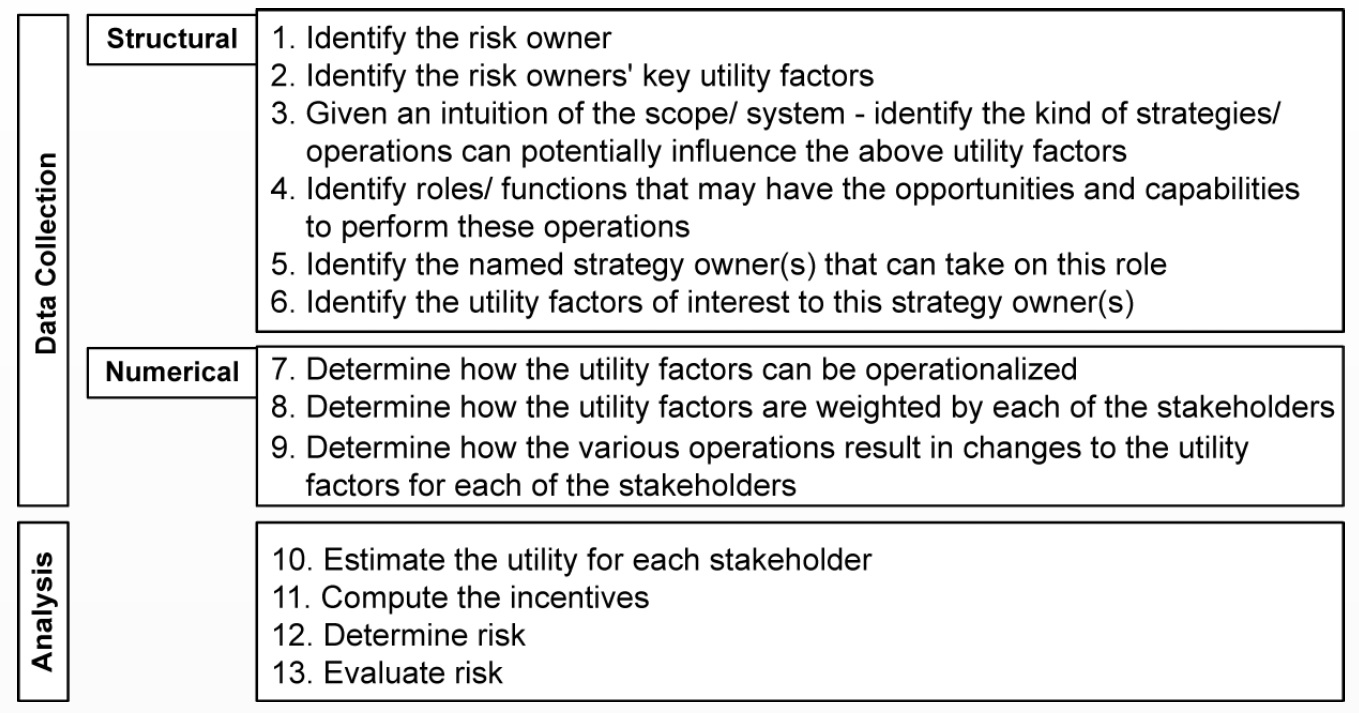
\includegraphics[width=0.8\textwidth]{Figure/CIRA_process.jpg}
  \caption{Procedure in CIRA, based on \cite{lisathesis}}
  \label{fig:CIRA_process}
\end{figure}


\section{Cloud Computing} \label{cloudcomp}
This section is based on the published work of the scientists at the U.S. National Institute of Standards and Technology (NIST) \cite{mell2011nist}.

Cloud computing can be defined as a model to provide ubiquitous, convenient, on-demand network access to a shared pool of configurable computing resources \cite{csaguide3.0}. It has the potential to increase collaboration, scalability, availability and agility. The main advantage of cloud computing is that it provides customers/users to pay per use facility \cite{6203873}. Customers do not need to pay for the infrastructure, software, installation of different hardwares and maintenance. NIST defines cloud computing (see Figure \ref{fig:cloud_visual_model}) as an aggregation of five essential characteristics (On-demand self-service, Broad network access, Resource pooling, Rapid elasticity, Measured Service); three service models (Cloud Software as a Service (SaaS), Cloud Platform as a Service (PaaS), Cloud Infrastructure as a Service (IaaS)); and, four deployment models (Private cloud, Community cloud, Public cloud, Hybrid cloud) \cite{mell2011nist}.

\begin{figure}[H]
	\centering
  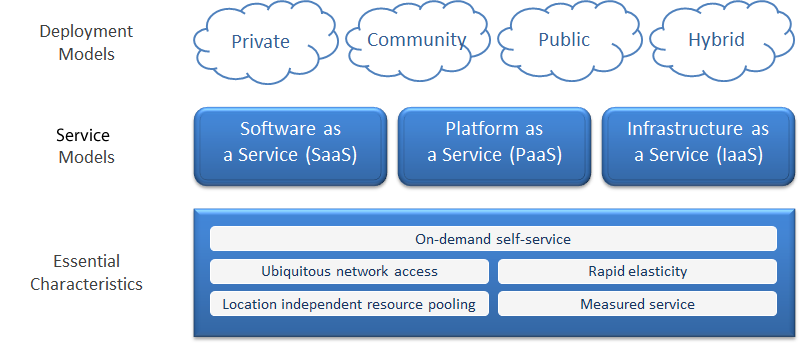
\includegraphics[width=0.8\textwidth]{Figure/visual_model.png}
  \caption{NIST Visual Model of Cloud Computing Definition, based on \cite{mell2011nist}}
  \label{fig:cloud_visual_model}
\end{figure}

\subsection{Essential Characteristics}

Cloud services possess five essential characteristics. These characteristics show how cloud computing is different from and related to traditional computing.
\begin{itemize}
\item \textbf{On-demand self-service -} A consumer can unilaterally provision computing capabilities, such as server time and network storage, as needed automatically without requiring human interaction with each service provider.

\item \textbf{Broad network access -} Capabilities are available over the network and accessed through standard mechanisms that promote use by heterogeneous thin or thick client platforms (e.g., mobile phones, tablets, laptops, and workstations).

\item \textbf{Resource pooling -} The provider's computing resources are pooled to serve multiple consumers using a multi-tenant model, with different physical and virtual resources dynamically assigned and reassigned according to consumer demand. There is a sense of location independence in that the customer generally has no control or knowledge over the exact location of the provided resources but may be able to specify location at a higher level of abstraction (e.g., country, state, or datacenter). Examples of resources include storage, processing, memory, and network bandwidth.

\item \textbf{Rapid elasticity -} Capabilities can be elastically provisioned and released, in some cases automatically, to scale rapidly outward and inward commensurate with demand. To the consumer, the capabilities available for provisioning often appear to be unlimited and can be appropriated in any quantity at any time.

\item \textbf{Measured service -} Cloud systems automatically control and optimize resource use by leveraging a metering capability at some level of abstraction appropriate to the type of service (e.g., storage, processing, bandwidth, and active user accounts). Resource usage can be monitored, controlled, and reported, providing transparency for both the provider and consumer of the utilized service.
\end{itemize}

\subsection{Service Models}

Cloud service delivery model is divided among three models. It is also known as SPI model where SPI refers to Software, Platform and Infrastructure respectively. 

\begin{itemize}
\item \textbf{Software as a Service (SaaS) -} The capability provided to the consumer is to use the provider's applications running on a cloud infrastructure. The applications are accessible from various client devices through either a thin client interface, such as a web browser (e.g., web-based email), or a program interface. The consumer does not manage or control the underlying cloud infrastructure including network, servers, operating systems, storage, or even individual application capabilities, with the possible exception of limited user-specific application configuration settings. Examples of multi tenant SaaS provision from cloud managed environments are Workday.com Inc and SalesForce.com Inc. Workday offersHR and Payroll software, whereas SalesForce.com offers Customer Relationship Management (CRM) software.

\item \textbf{Platform as a Service (PaaS) -} The capability provided to the consumer is to deploy onto the cloud infrastructure consumer-created or acquired applications created using programming languages, libraries, services, and tools supported by the provider. The consumer does not manage or control the underlying cloud infrastructure including network, servers, operating systems, or storage, but has control over the deployed applications and possibly configuration settings for the application-hosting environment. Prominent examples of PaaS are Google AppEngine \cite{googleapp} and SalesForce.com's business software development's platform.

\item \textbf{Infrastructure as a Service (IaaS) -} The capability provided to the consumer is to provision processing, storage, networks, and other fundamental computing resources where the consumer is able to deploy and run arbitrary software, which can include operating systems and applications. The consumer does not manage or control the underlying cloud infrastructure but has control over operating systems, storage, and deployed applications; and possibly limited control of select networking components (e.g., host firewalls). The most notable IaaS cloud offerings appear to be Amazon's e.g. Elastic Compute cloud (EC2) \cite{amazonec2}, GoGrid's cloud Hosting/ Storage \cite{gogrid}. 

\end{itemize}

\iffalse
\subsection{Deployment Models}

There are four deployment models for cloud services to address specific requirements. The choice of deployment is not related to the choice of the service model.

\begin{itemize}
\item \textbf{Private cloud -} The cloud infrastructure is provisioned for exclusive use by a single organization comprising multiple consumers (e.g., business units). It may be owned, managed, and operated by the organization, a third party, or some combination of them, and it may exist on or off premises.

\item \textbf{Community cloud -} The cloud infrastructure is provisioned for exclusive use by a specific community of consumers from organizations that have shared concerns (e.g., mission, security requirements, policy, and compliance considerations). It may be owned, managed, and operated by one or more of the organizations in the community, a third party, or some combination of them, and it may exist on or off premises.

\item \textbf{Public cloud -} The cloud infrastructure is provisioned for open use by the general public. It may be owned, managed, and operated by a business, academic, or government organization, or some combination of them. It exists on the premises of the cloud provider.

\item \textbf{Hybrid cloud -} The cloud infrastructure is a composition of two or more distinct cloud infrastructures (private, community, or public) that remain unique entities, but are bound together by standardized or proprietary technology that enables data and application portability (e.g., cloud bursting for load balancing between clouds).
\end{itemize}

\fi

\section{Security and Privacy issues}\label{SecAndPrivacy}

The U.S. information technology research and consulting firm Gartner issued a report in 2008 \cite{Gartner}. This report was based on mainly from the vendor's point of view about security capabilities analyzed security risks faced by the cloud. Table \ref{tab:Gartner} lists seven major security risks that are common in any cloud computing environment.

\begin{table}[h]
	\centering
		\begin{tabular}{|p{4cm}|p{9cm}|}\hline
		
		\textbf{Risk} & \textbf{Description} \\ 
	\hline			
		Privileged user access & Sensitive data processed outside the enterprise brings with it an inherent level of risk. \\ \hline
		Regulatory compliance & Customers are ultimately responsible for the security and integrity of their own data, even when it is held by a service provider. \\ \hline
		Data location & When you use the cloud, you probably won't know exactly where your data is hosted. \\ \hline
		Data segregation & Data in the cloud is typically in a shared environment alongside data from other customers. \\ \hline
		 Recovery & Any offering that does not replicate the data and application infrastructure across multiple sites is vulnerable to a total failure. \\ \hline
		 Investigative support & Investigating inappropriate or illegal activity may be impossible in cloud computing \\ \hline
		 Long-term viability & you must be sure your data will remain available even after such an event. \\ \hline \hline
		
		\end{tabular}
	\caption{Gartner: Seven cloud-computing security risks, based on \cite{Gartner}}
	\label{tab:Gartner}
\end{table}

La'Quata Sumter \cite{Sumter:2010:CCS:1900008.1900152} stated the wide adoption of cloud computing and its concerns related to Internet security. Consumers of cloud computing services have serious concern about the availability and accessibility of their data in the cloud. A mechanism is proposed to ensure the safety and security of data. This design helps to capture the movement and processing of the information kept on the cloud. The proposed mechanism is implemented in a small cloud computing environment. The major advantage of the research work is the assurance of security to cloud users but at the same time the proposed design is not feasible for large scale cloud computing environments.

Soren et al \cite{Bleikertz:2010:SAM:1866835.1866853} stated that cloud computing has gained popularity in recent years but the benefits of clouds are shadowed by security and privacy challenges. These challenges are also affecting the adoption of cloud service in any company. Users can configure highly flexible cloud computing environment through a web services interface. However, misconfiguration of any cloud service can impose severe vulnerability in the system. Authors presented a novel approach for analyzing security at end user configuration. Amazon Elastic compute cloud (EC2) is selected for the security assessment. The focus of the assessment is on the reachability and vulnerability of services in cloud infrastructure. A query and policy language is also proposed in this paper for the analysis. It can be used to understand necessary and unnecessary configuration. This approach enables to remediate common security concerns through validation of configurations of complex cloud infrastructures. The major benefit of this approach is that it provides analysis of vulnerability and security issues. This analysis is helpful for the vendors as they can improve their security policies based on the analysis. The potential drawback of this scheme is its limitation to Amazon \cite{6148380}.

Flavi and Roberto \cite{Lombardi:2010:TSC:1774088.1774176} reported that clouds environments are becoming prominent targets for attackers. This paper discusses the integrity problem in the clouds and propsed a new architecture to increase security of cloud resources. They named it as Transparent Cloud Protection System (TCPS). The main idea of TCPS system is that it can be customized to different cloud environments to monitor the integrity of guests and infrastructure components while remaining transparent to virtual machines. The proposed tool improves security, transparency and intrusion detection mechanism. The major drawback of their work is that the proposed tool is not deployed or tested in any cloud computing scenario.

\chapter{Research Methodology (2 - 4p)}\label{ResMethod}

According to \cite{Hevner:2004:DSI:2017212.2017217}, there are two distinct paradigm to acquire knowledge in Information System viz. behavioral science and design science. Behavioral science paradigm is based on natural science research methods. It seeks to develop and justify theories that explain human-organizational interaction phenomenon surrounding the analysis, design, implementation, management, and use of information systems. On the other hand, Design science is fundamentally a problem- solving paradigm and based on engineering. It seeks to create innovations that define the ideas, practices, technical capabilities, and products through which the analysis, design, implementation, management, and use of information systems can be effectively and efficiently accomplished.

The aim of this research is to solve an existing practical problem in the realm of risk analysis tools by creating an artifact based on the existing theories of  CIRA tool and cloud services. The problem will be solved by applying creativity, innovation and problem solving capabilities. The created artifact would then be practically applied to bridge the gap between risk analysis modeling and design of cloud service to support the business. Thus, the research clearly lies in the domain of design science research in information systems.

\section{Design Science}\label{DesignSc}

Design science research, which is popular in disciplines such as engineering and architecture, focuses on creation: ``how things ought to be in order to attain goals, and to function''. The purpose of design is to change existing situations into preferred ones. The fundamental principle of Design science research is based on seven guidelines. The important guidelines provided by \cite{Hevner:2004:DSI:2017212.2017217} are as follows:

\begin{itemize}
	\item Design science research must result in creation of an innovative and practical artifact.
	\item It must provide solution to practical problem of a Business.
	\item The artifact must be evaluated and verified according to the specified problem
	\item The artifact must be novel in nature i.e. it must solve an unsolved problem or a solved problem in an effective way.
	\item Design science research must be based on the application of rigorous methods in both the construction and evaluation of the design artifact
	\item The research is an iterative search process where available resources are used to achieve desired goals while maintaining the environmental constraints.
	\item The outcome of the research work must be communicated to both managerial and technical audience.
\end{itemize}

The DSR process includes six steps: problem identification and motivation, definition of the objectives for a solution, design and development, demonstration, evaluation, and communication. The arrows on the left side of \ref{fig:DSR_steps} emphasize the importance of iteration as part of the DSRM. They show that activities such as Evaluation and Communication often result in revising the artifact's objectives and design. Iteration is ingrained in design science research and \cite{Hevner:2004:DSI:2017212.2017217} illustrate that with their build-and-evaluate loop: evaluation provides feedback information on the designed artifact and a better understanding of the problem which leads to a re-iteration of the design process. 
Table \ref{tab:DSRMCIRA} describes DSR process in case of CIRA cloud service.

\begin{figure}[h]
	\centering
  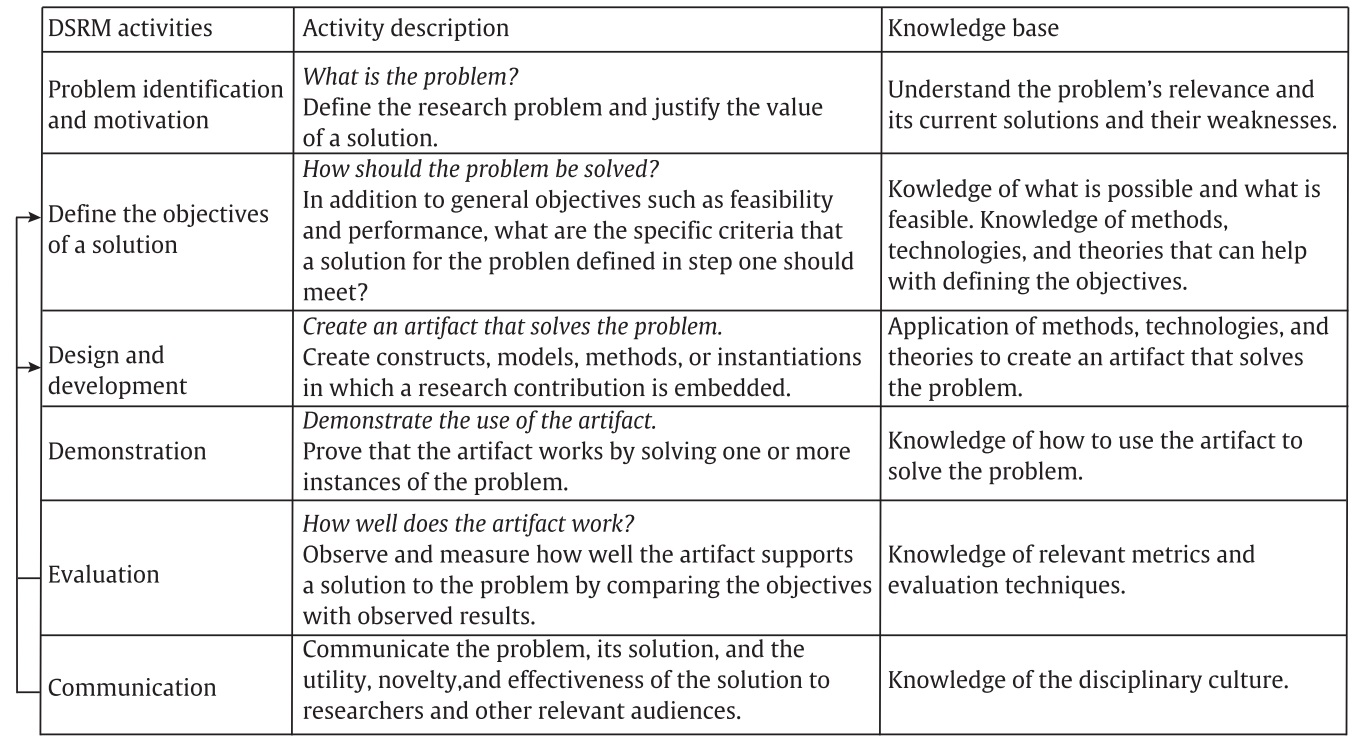
\includegraphics[width=0.8\textwidth]{Figure/process.jpg}
  \caption{Steps in Design Science Research, based on \cite{Geerts2011142}}
  \label{fig:DSR_steps}
\end{figure}

\begin{table}[h]
	\centering
		\begin{tabular}{|p{0.4cm}|p{3cm}|p{5cm}|p{5cm}|}\hline
		
		\textbf{No.} & \textbf{DSRM Activites} & \textbf{Activity Description} & \textbf{Knowledge Base} \\ 
	\hline			
				1 & Problem identification and motivation & The risk analysis methods need to be extended to broader spectrum of information management to ensure secure and efficient data collection, data sharing and data operation service & Literature review of studies that discuss weakness of various risk analysis methods: report published by the OCTAVE, CORAS and a series of research paper that explore the different approaches to make risk analysis method more effective. \\ \hline
				2 & Define the objectives of a solution & Design of a system that is secure and it can achieve economies of scale, globalize the workforce, reduce capital cost of implement CIRA risk analysis method in a company. & Knowledge of distributed and cloud computing and their security and privacy issues. \\  \hline
				3 & Design and Development & Design of CIRA cloud service model: a framework to be used in a shared data environment where both experts and non-experts can contribute in risk analysis. & Cloud computing, CIRA methods, service oriented architecture, vCloud api programming, security engineering. \\ \hline
				4 & Demonstration & Formation of several instances of the problem to understand the effectiveness of the designed framework & Applying CIRA cloud service to real world problems. \\ \hline
				5 & Evaluation & CIRA cloud service must be evaluated in terms of scalability, security and operation cost? & Definition of performance measures and security metrics. \\ \hline				
				6 & Communication & The work shall be published in relevant conferences and journals. & List of all related conferences and journals according to the impact factors and relevance to the topic. \\ \hline
				\hline
				
		\end{tabular}
	\caption{DSRM applied to CIRA as a cloud service.}
	\label{tab:DSRMCIRA}
\end{table}

Design science research can be seen as an embodiment of three closely related cycles of activities \ref{fig:DSR_cycles}. The Relevance Cycle bridges the contextual environment of the research project with the design science activities. The Rigor Cycle connects the design science activities with the knowledge base of scientific foundations, experience, and expertise that informs the research project. The central Design Cycle iterates between the core activities of building and evaluating the design artifacts and processes of the research. \cite{Hevner:2004:DSI:2017212.2017217} Suggest that design science research should address either an unsolved problem in a unique and innovative way or a solved problem in a more effective or efficient way.

\begin{figure}[H]
	\centering
	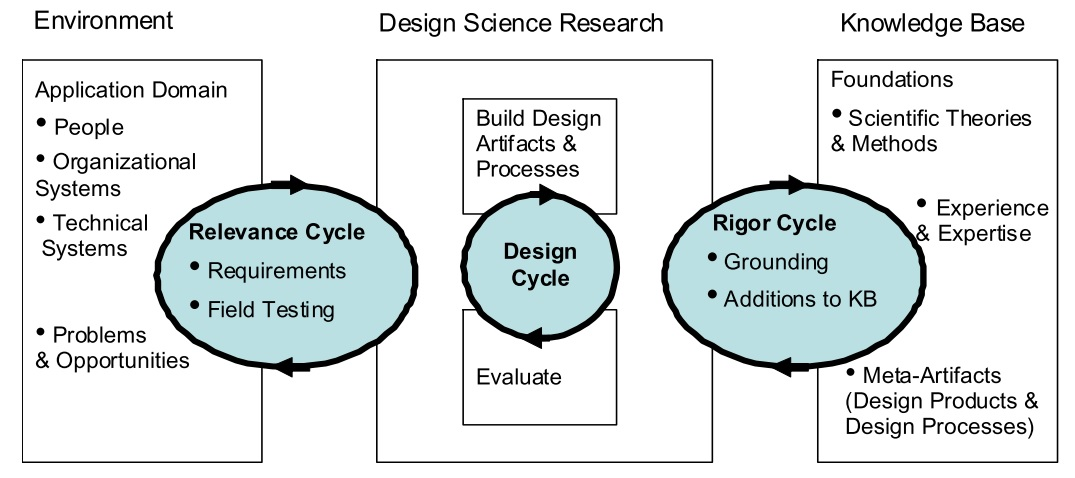
\includegraphics[width=0.8\textwidth]{Figure/DSR.jpg}
	\caption{cycles of Design Science Research}
	\label{fig:DSR_cycles}
\end{figure}

\section{Methods and research questions}\label{Methods}

\begin{enumerate}
\item \textbf{RQ1}: What are the quality and cost effective improvement features of CIRA tool as a cloud delivery model?

\textbf{Related to:} Define the objectives of a solution, design and development

\textbf{Research Method and Strategy:} Case study will be used as the research method to investigate the possible improvement features. 

\textbf{Data Collection Method:} Data required to investigate this research work will be collected from the literature review of various existing cloud delivery and risk analysis models. The detailed information of these models can be fetched from major databases such as IEEE computer society, CiteseerX, ACM digital library etc.. 

\item \textbf{RQ2}: What are the security requirements of an information sharing tool?

\textbf{Related to:} Define the objectives of a solution, design and development 

\textbf{Research Method and Strategy:} case study 

\textbf{Data Collection Method:} literature surveys

\item \textbf{RQ3}: What kind of information sharing features can be of special interest for the participants?

\textbf{Related to:} Define the objectives of a solution, design and development

\textbf{Research Method and Strategy:} Case study 

\textbf{Data Collection Method:}

\item \textbf{RQ4}: How can the desired functionality be implemented without violating the security requirements?

\textbf{Related to:} design and development

\textbf{Research Method and Strategy:} Process modelling

\textbf{Data Collection Method:}

\item \textbf{RQ5}: What are the benefits and shortcomings of the newly implemented features in the CIRA support tool?

\textbf{Related to:} Design demonstration and Design evaluation

\textbf{Research Method and Strategy:} Experimentation

\textbf{Data Collection Method:}

\item What is impact of the security risks and shortcomings of the added feature on adoption of cloud computing?

\textbf{Related to:} Design evaluation

\textbf{Research Method and Strategy:}

\textbf{Data Collection Method:}

\end{enumerate}

\chapter{Milestone}\label{milestone}

\begin{table}[H]
	\centering
		\begin{tabular}{|c|c|c|c|c|} \hline 
			\textbf{semester} & \textbf{code} & \textbf{Title} & \textbf{ECTS} & \textbf{Institute} \\ \hline
			
			\multirow{3}{*}{Spring'14} & IMT 6261 & Scientific Communication & 5 & GUC \\
																&IMT 6011 & Introduction to information security & 5 & GUC \\
																&IMT 6221 & Mobile Technology & 5 & GUC\\
																\hline
																
		 \multirow{3}{*}{Autumn'14} & IMT 6001 & Ethics and legal aspects of scientific research & 5 & GUC \\
																&IMT 6111 & Risk management I & 5 & GUC \\
																&IMT 6061 & Risk management II & 5 & GUC \\
																\hline				\hline											
																
		\end{tabular}
	\caption{Overview of PhD courses}
	\label{tab:OverviewOfPhDCourses}
\end{table}

\section{External Institution}\label{ExtInst}

As my PhD research area is related to risk analysis, cloud computing and security engineering, I will target research groups who are working on the implementation of the cloud services, risk analysis, security in software engineering. I have identified few research teams and organizations that are working remarkable research work in the field of cloud computing. The first one is the FP7 Marie Curie Initial Training Network RELATE group. \url{http://www.relate-itn.eu/}. The other one is IBM zurich computer science department. They are mainly working on the security aspects of cloud ccomputing. \url{http://www.zurich.ibm.com/csc/security/securevirt.html}. I will start communicating these groups after the approval of my research proposal.


\section{Paper publications (<2 p)}\label{PaperPub}

\begin{enumerate}
\item Limitations of Risk analysis models
\item Evaluation of risk analysis methods in the context of cloud service
\item Impact of security issues on the adoption of cloud computing in Conflicting Incentives Risk analysis method
\item Evaluation of security controls to mitigate adoption risk  of CIRA to cloud environment.
\item security metrics for CIRA cloud service.
\end{enumerate}

\section{Research Risk and Mitigation (< 2 p)}\label{ResRiskMit}

\textbf{Data Availability}

The concept of this research work is based on the idea of cloud computing and risk analysis methods focusing mainly on the security and privacy aspects of it. The concept of cloud computing and CIRA is new and several issues are still unsolved or unconsidered. I will consider data published in the reports of companies like IBM, AMAZON, SalesForce. These companies are doing remarkable research work in the field of cloud computing.

\textbf{Paper rejection}

There is always a risk associated with the paper being submitted to a conference or journal. A paper may be rejected due to the low acceptance rate of the conference or because of very high impact factor value. If my paper gets rejected due to any reason, I will discuss the issue with my supervisors so that I can address the shortcoming of the paper and resubmit in other relevant conferences.

\section{Conferences and Journals}\label{Confpub}

\begin{itemize}

	\item Security \& Privacy	
	\begin{itemize}
		\item IEEE International Conference on Trust, Security and Privacy in Computing and Communications
		\item International Conference on Security and Privacy in Communication Networks
		\item International Conference on Informatics and Information Technology
		International Workshop on Software Engineering for the Smart Grid
	\end{itemize}
	
	\item Security Management
	\begin{itemize}
		\item Disaster, Risk and Vulnerability Conference 2014
		\item IEEE Colloquium on Risk Analysis Methods and Tools
		\item SRA Journal
		\item Conference on Cloud Security Management
		\item 11th International Workshop on Security in Information Systems 
	\end{itemize}
	
	\item Cloud Computing
	\begin{itemize}
		\item The ACM Cloud Computing Security Workshop
		\item IEEE International Conference on Cloud Computing
		\item IEEE International workshop on Cloud Computing Applications and SEcurity
		\item IEEE International Conference on Cloud Computing Technology and Science
		The Second International Conference on Digital Information Processing, E-Business and Cloud Computing (DIPECC 2014)
	\end{itemize}
	
	\item Information Sciences	
	\begin{itemize}
		\item Journal of Emerging Trends in Computing and Information Sciences 
	\end{itemize}
	
\end{itemize}


\chapter{Supervision}\label{supervision}
For this project I propose Dr. Einar Arthur Snekkenes, Professor, NISLab as my principal supervisor

\chapter{Funding Plan}\label{Fund}
The source is internal funding of NISLAB.

\chapter{Ethical and legal considerations}\label{Ethics}

I shall follow the ethical guidelines as published in Guidelines for Research Ethics in Science and Technology by The National Committee for Research Ethics in Science and Technology, Norway (NENT) 

\textbf{Good Publication practice}

I shall follow good Publication practice. I shall denote all the source material and respects the original contributions of others through citations. Honorary authorships are unacceptable. Rightful authorship is considered to be defined by three criteria:

\begin{enumerate}
	\item All the authors must have made a significant and directly academic contribution to at least two of the four components of a typical research project:	
	
	\begin{enumerate}
		\item concept or design
		
		\item Data collection and processing
		
		\item Analysis and interpretation of data
		
		\item Written formulation of substantial parts of the work
		
	\end{enumerate}
\item All the authors should have critically read through the different drafts and approved the final version

\item All the authors should be capable of defending the work in its entirety (though not necessarily all the technical details).

\end{enumerate}

\textbf{Honest research practices}

\begin{itemize}
	\item I shall follow Integrity, honesty and accountability while conducting my research work.
	
	\item I shall not follow any scientific fraudulence, either in the form of forgery, manipulation or the selective presentation of data from research con- ducted by themselves or others
	
	\item I shall not indulge in plagiarism of research.
	
	\item I shall make data accessible to others for verification.
	
	\item I shall present research done by others in a balanced and honest manner.
	
\end{itemize}

\textbf{Statement of Compliance}

\textit{I will conduct my activities as a researcher with integrity and honesty; I will use my sci- entific knowledge and skills for the benefit of humanity and for a sustainable development; I will show respect for animals and nature; I will act in accordance with research ethics, and I will not allow considerations based on ideology, religion, ethnicity, prejudices or material advantages to overshadow my ethical responsibility as a researcher.}
 
%% <== End of hints
%%%%%%%%%%%%%%%%%%%%%%%%%%%%%%%%%%%%%%%%%%%%%%%%%%%%%%%%%%%%%



%%%%%%%%%%%%%%%%%%%%%%%%%%%%%%%%%%%%%%%%%%%%%%%%%%%%%%%%%%%%%
%% BIBLIOGRAPHY AND OTHER LISTS
%%%%%%%%%%%%%%%%%%%%%%%%%%%%%%%%%%%%%%%%%%%%%%%%%%%%%%%%%%%%%
%% A small distance to the other stuff in the table of contents (toc)
\addtocontents{toc}{\protect\vspace*{\baselineskip}}

%% The Bibliography
%% ==> You need a file 'literature.bib' for this.
%% ==> You need to run BibTeX for this (Project | Properties... | Uses BibTeX)
%\addcontentsline{toc}{chapter}{Bibliography} %'Bibliography' into toc
%\nocite{*} %Even non-cited BibTeX-Entries will be shown.
%\bibliographystyle{alpha} %Style of Bibliography: plain / apalike / amsalpha / ...
%\bibliography{literature} %You need a file 'literature.bib' for this.

%% The List of Figures
%\clearpage
%\addcontentsline{toc}{chapter}{List of Figures}
%\listoffigures
%
%%% The List of Tables
%\clearpage
%\addcontentsline{toc}{chapter}{List of Tables}
%\listoftables

\clearpage
\addcontentsline{toc}{chapter}{Bibliography}
\bibliography{../../Latex/CIRA_ClOUD/literature}
\bibliographystyle{ieeetr}


%%%%%%%%%%%%%%%%%%%%%%%%%%%%%%%%%%%%%%%%%%%%%%%%%%%%%%%%%%%%%
%% APPENDICES
%%%%%%%%%%%%%%%%%%%%%%%%%%%%%%%%%%%%%%%%%%%%%%%%%%%%%%%%%%%%%
%\appendix
%\appendix
%% ==> Write your text here or include other files.

%\input{FileName} %You need a file 'FileName.tex' for this.


\end{document}

